\documentclass[unicode]{beamer}

\usepackage{luatexja}
\usepackage[ipaex]{luatexja-preset}
\usepackage{graphicx, color}
\usepackage{hyperref}
\usepackage{listings}
\usepackage{caption}
\usepackage{tikz}
\usepackage{amsmath,amssymb,nccmath}
\usepackage{overpic}

\usetikzlibrary{arrows}
\usetikzlibrary{arrows.meta}
\usetikzlibrary{positioning}

\lstset{
    language=Scala,
    breaklines=true,
    breakindent=10pt,
    basicstyle=\ttfamily\scriptsize,
    commentstyle={\itshape},
    keywordstyle={\bfseries\color[rgb]{0,0,1}},
    frame = tbl,
    numbers = left,
    stepnumber = 1,
    numberstyle = \tiny,
    tabsize = 4
}

\captionsetup{font={footnotesize}}

\setbeamertemplate{footline}[frame number]

\title{Chisel を用いたエッジ検出フィルタの実装とVivado HLSとの比較}
\author{佐々木 隆汰}
\date{December 2020}

\begin{document}

\begin{frame}{}
    \maketitle
\end{frame}

\begin{frame}{Contents}
   \begin{itemize}
       \item Chisel の導入
       \item Pros. \& Cons.
       \item ChiselImProc の説明
       \item Vivado HLS との比較
   \end{itemize} 
\end{frame}


\begin{frame}{Contents}
   \begin{itemize}
       \item[\textcolor{red}{$\rhd$}] Chisel の導入
       \item Pros. \& Cons.
       \item ChiselImProc の説明
       \item Vivado HLS との比較
   \end{itemize} 
\end{frame}


\begin{frame}{Chisel の導入}
    \begin{itemize}
        \item JDK とsbt を導入 \\
            (\url{https://www.scala-sbt.org/})
        \item chisel-template をclone \\
            (\url{https://github.com/freechipsproject/chisel-template})
            
        \item プロジェクト名をリネーム
    \end{itemize}
    
\end{frame}

\begin{frame}[fragile]{Chisel の文法}

    \begin{itemize}
        \item 各モジュールはModuleクラスを拡張して作成。
        \begin{lstlisting}[language=Scala,caption={Lチカモジュール}]
class Hello extends Module {
     val io = IO(new Bundle {
        val led = Output (UInt (1.W))
     })
     val CNT_MAX = (50000000 / 2 - 1).U;
     
     val cntReg = RegInit(0.U(32.W))
     val blkReg = RegInit(0.U(1.W))
     
     cntReg := cntReg + 1.U
     when (cntReg === CNT_MAX) {
        cntReg := 0.U
        blkReg := ~blkReg
     }
     io.led := blkReg
}
        \end{lstlisting}
    \end{itemize}
    
\end{frame}



\begin{frame}[fragile]{信号型と定数}
    \begin{itemize}
        \item ビットのベクトルを表す3つのデータ型。
            \begin{lstlisting}
Bits(8.W)
UInt(8.W)
SIng(8.W)
            \end{lstlisting}
        \item データ幅はWidth型で表す。
        \item 定数データを記述するときはメソッド呼び出しを用いる。
            \begin{lstlisting}
8.U(4.W)    // ビット幅は引数で指定
0.U
-3.S        // ビット幅は指定しなくても推論してくれる
            \end{lstlisting}
        \item 論理型(UInt(1.W)の拡張)
            \begin{lstlisting}
Bool()
true.B
false.B
            \end{lstlisting}
    \end{itemize} 
\end{frame}


\begin{frame}[fragile]{組み合わせ回路}
   \begin{itemize}
       \item 論理演算子
       \begin{lstlisting}
val and = a & b    // bitwise and
val or = a | b     // bitwise or
val xor = a ^ b    // bitwise xor
val not = ~a       // bitwise negation
       \end{lstlisting}
       
       \item 算術演算子
       \begin{lstlisting}
val add = a + b
val sub = a - b
val neg = - a
val mul = a * b
val div = a / b
val mod = a % b
       \end{lstlisting}
   \end{itemize} 
\end{frame}



\begin{frame}[fragile]{組み合わせ回路}
    \begin{itemize}
        \item 信号タイプを先に定義してから、更新演算子を使用して
        信号に値を割り当てることもできる。
        \begin{lstlisting}
val w = Wire (UInt())
w := a & b
        \end{lstlisting}
        
        \item 1ビットの抽出
        \begin{lstlisting}
val sign = x(31)
        \end{lstlisting}
        
        \item 範囲指定で抜き出し
        \begin{lstlisting}
val lowByte = largeWord(7, 0)
        \end{lstlisting}
        
        \item 信号の結合
        \begin{lstlisting}
val word = Cat(highByte, lowByte)
        \end{lstlisting}
    \end{itemize}
\end{frame}



\begin{frame}[fragile]{組み合わせ回路}
    \begin{itemize}
        \item マルチプレクサ
        \begin{lstlisting}
val y = Mux (sel, a, b)
        \end{lstlisting}
        \begin{figure}[h]
            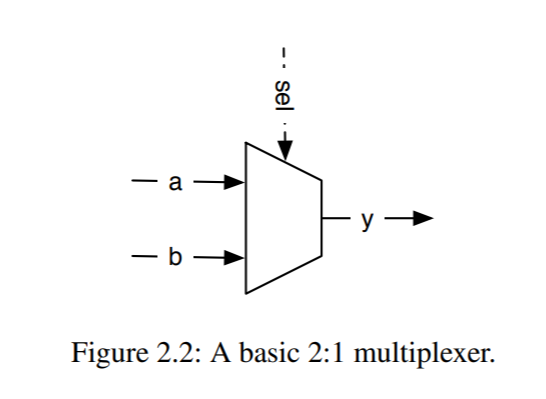
\includegraphics[width=0.5\textwidth]{./figures/mux.png}
        \end{figure}
    \end{itemize}
\end{frame}



\begin{frame}[fragile]{レジスタ}
    \begin{itemize}
        \item リセット時に0で初期化される8ビットレジスタ
        \begin{lstlisting}
val reg = RegInit(0.U(8.W))
reg := d                    // 更新演算子で更新
val q = reg                 // レジスタの値を取り出す
        \end{lstlisting}
        
        \item 初期値が不定(X)のレジスタ
        \begin{lstlisting}
val reg = Reg(UInt(8.W))
        \end{lstlisting}
        
        \item カウンター
        \begin{lstlisting}
val cntReg = RegInit(0.U(8.W))
cntReg := Mux (cntReg === 9.U, 0.U, cntReg + 1.U)
        \end{lstlisting}
    \end{itemize}
    
\end{frame}



\begin{frame}[fragile]{Bundle と Vec}
    \begin{itemize}
        \item Bundle: 異なるタイプの複数の信号をまとめる。
        \begin{lstlisting}
class Channel() extends Bundle {
    val data = UInt(32.W)
    val valid = Bool()
}
        \end{lstlisting}
        
        \item フィールドにはドット表記でアクセス。
        \begin{lstlisting}
val ch = Wire (new Channel())
ch.data := 123.U            // 更新演算子で更新できる
ch.valid := true.B          // 更新演算子で更新できる
val b = ch.valid            // フィールドだけを参照
val channel = ch            // 全体を参照
        \end{lstlisting}
        
        \item Vec: 同じタイプの複数の信号をまとめる。
        \begin{lstlisting}
val v = Wire (Vec (3, UInt(4.W)))
v(0) := 1.U                 // アクセスは配列と同じ
v(1) := 3.U                 // アクセスは配列と同じ
v(2) := 5.U                 // アクセスは配列と同じ
        \end{lstlisting}
    \end{itemize}
    
\end{frame}




\begin{frame}[fragile]{テスト}
    PeekPokeTesterでIOポートからデータを入出力できる
    \begin{lstlisting}
class DeviceUnderTest extends Module {
    val io = IO (new Bundle {
        val a = Input (UInt(32.W))
        val b = Input (UInt(32.W))
        val out = Output (UInt(2.W))
    })
    io.out := io.a & io.b
}
    \end{lstlisting}
    
    \begin{lstlisting}
class TesterSimple (dut: DeviceUnderTest) 
        extends PeekPokeTester(dut) {
    poke (dut.io.a, 0.U)
    poke (dut.io.b, 1.U)
    step (1)
    println ("Result is: " + peek(dut.io.out).toString)
    poke (dut.io.a, 4.U)
    poke (dut.io.b, 2.U)
    step (1)
    expect (dut.io.out, 0)
}
    \end{lstlisting}

    
\end{frame}



\begin{frame}{Contents}
   \begin{itemize}
       \item[\textcolor{red}{$\checkmark$}] Chisel の導入
       \item[\textcolor{red}{$\rhd$}] Pros. \& Cons.
       \item ChiselImProc の説明
       \item Vivado HLS との比較
   \end{itemize} 
\end{frame}



\begin{frame}{Pros. \& Cons.}
            \begin{block}{Pros.}
                \begin{itemize}
                    \item OOP の強みは大体使える。
                    \item 型パラメータを利用できる。
                    \item 再利用性は高い。
                    \item 出力されたvファイルと元のScalaのコードの対応が見やすい。
                    
                \end{itemize}
            \end{block}
            \begin{block}{Cons.}
                \begin{itemize}
                    \item クロックは常に意識しないと厳しい。
                    \item AXI はchisel3だと結局ない(?)
                    \item vファイルがやたら重い。
                    \item XRESETには対応していない。
                \end{itemize}
            \end{block}
    
\end{frame}

\begin{frame}[fragile]{AXI Stream}
    \begin{itemize}
        \item 型パラメータを利用できる。
        \item 上限境界 (<:) なども利用できる。
        \begin{lstlisting}[caption={"AXI Stream Interface"}]
class AXIStreamIF[T <: Data](gen: T) 
        extends ReadyValidIO[T](gen) {
    val user = Output (Bool())
    val last = Output (Bool())

    override def cloneType: this.type 
        = new AXIStreamIF(gen).asInstanceOf[this.type]
}

object AXIStreamMasterIF {
    def apply [T <: Data] (gen: T): AXIStreamIF[T] 
        = new AXIStreamIF[T] (gen)
}

object AXIStreamSlaveIF {
    def apply [T <: Data] (gen: T): AXIStreamIF[T] 
        = Flipped (new AXIStreamIF[T] (gen))
}            
        \end{lstlisting}
        
        \item Data 型はChisel のすべてのデータのsupertype
    \end{itemize}
    
\end{frame}




\begin{frame}{Data Types Overview}
    \begin{figure}[h]
        \centering
        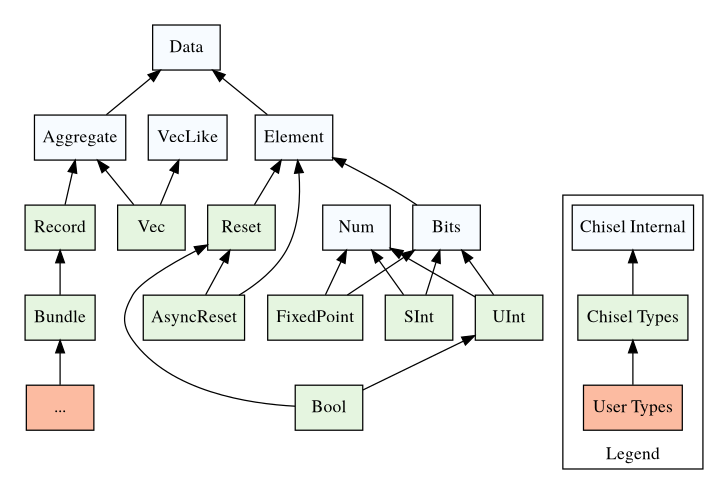
\includegraphics[width=\textwidth]{./figures/type_hierarchy.png}
    \end{figure}
\end{frame}



\begin{frame}[fragile]{AXI Streamを用いたモジュール}
    \begin{lstlisting}
class FifoAXIStreamDIO[T <: Data, U <: Data] (
    private val genEnq: T,
    private val genDeq: U
) extends Bundle {
    val enq = AXIStreamSlaveIF(genEnq)
    val deq = AXIStreamMasterIF(genDeq)
}

class FifoAXIStreamIO[T <: Data] (private val gen: T)
        extends FifoAXIStreamDIO(gen, gen) {
}

abstract class FifoAXIS[T <: Data] (gen: T, depth: Int)
        extends Module {
    val io = IO (new FifoAXIStreamIO[T] (gen))
    assert (depth > 0, 
        "Number of buffer elements needs to be larger than 0")
}
    \end{lstlisting}
    
    ※ enq と deq は Chiselと僕のコードで逆。
\end{frame}

\begin{frame}[fragile]{積和モジュール}

\begin{itemize}
    \item 8bit で3x3は遅延しない(1クロックで動作できる)
    \item 8bit で5x5は遅延する(1クロックで動作できない)
    \item 16bit で3x3は遅延?
\begin{lstlisting}
class MulAdd (dataWidth: Int, num: Int) extends Module {
    val io = IO(new Bundle {
        val a = Input (Vec(num, UInt(dataWidth.W)))
        val b = Input (Vec(num, UInt(dataWidth.W)))
        val output = Output (UInt ((2*dataWidth).W))
    })

    var i = 0
    var tmp = 0.U((2*dataWidth).W)
    val step = 3                // 8bit で3x3は遅延しない
    for (i <- 0 until num by step) {
        var intmp = 0.U((2*dataWidth).W)
        for (j <- 0 until step) {
            intmp += io.a(i+j) * io.b (i+j)
        }
        tmp += intmp
    }
    io.output := tmp    
}
\end{lstlisting}
\end{itemize}
    
\end{frame}



\begin{frame}[fragile]{Verilogファイル生成}
    \begin{itemize}
        \begin{lstlisting}[language={Verilog}, basicstyle={\tiny}]
module MulAdd(
  input  [7:0]  io_b_0,
  input  [7:0]  io_b_1,
  input  [7:0]  io_b_2,
  input  [7:0]  io_b_3,
  input  [7:0]  io_b_4,
  input  [7:0]  io_b_5,
  input  [7:0]  io_b_6,
  input  [7:0]  io_b_7,
  input  [7:0]  io_b_8,
  output [15:0] io_output
);
  wire [15:0] _T = 8'h1 * io_b_0; // @[ChiselImProc.scala 32:32]
  wire [16:0] _T_1 = {{1'd0}, _T}; // @[ChiselImProc.scala 32:19]
  wire [15:0] _T_3 = 8'h2 * io_b_1; // @[ChiselImProc.scala 32:32]
  wire [15:0] _T_5 = _T_1[15:0] + _T_3; // @[ChiselImProc.scala 32:19]
  wire [15:0] _T_6 = 8'h1 * io_b_2; // @[ChiselImProc.scala 32:32]
  wire [15:0] _T_8 = _T_5 + _T_6; // @[ChiselImProc.scala 32:19]
  wire [16:0] _T_9 = {{1'd0}, _T_8}; // @[ChiselImProc.scala 34:13]
  wire [15:0] _T_11 = 8'h2 * io_b_3; // @[ChiselImProc.scala 32:32]
  wire [16:0] _T_12 = {{1'd0}, _T_11}; // @[ChiselImProc.scala 32:19]
  wire [15:0] _T_14 = 8'h4 * io_b_4; // @[ChiselImProc.scala 32:32]
  wire [15:0] _T_16 = _T_12[15:0] + _T_14; // @[ChiselImProc.scala 32:19]
  wire [15:0] _T_17 = 8'h2 * io_b_5; // @[ChiselImProc.scala 32:32]
  wire [15:0] _T_19 = _T_16 + _T_17; // @[ChiselImProc.scala 32:19]
  wire [15:0] _T_21 = _T_9[15:0] + _T_19; // @[ChiselImProc.scala 34:13]
  wire [15:0] _T_22 = 8'h1 * io_b_6; // @[ChiselImProc.scala 32:32]
  wire [16:0] _T_23 = {{1'd0}, _T_22}; // @[ChiselImProc.scala 32:19]
  wire [15:0] _T_25 = 8'h2 * io_b_7; // @[ChiselImProc.scala 32:32]
  wire [15:0] _T_27 = _T_23[15:0] + _T_25; // @[ChiselImProc.scala 32:19]
  wire [15:0] _T_28 = 8'h1 * io_b_8; // @[ChiselImProc.scala 32:32]
  wire [15:0] _T_30 = _T_27 + _T_28; // @[ChiselImProc.scala 32:19]
  assign io_output = _T_21 + _T_30; // @[ChiselImProc.scala 36:15]
endmodule
        \end{lstlisting}
    \end{itemize}
    
\end{frame}



\begin{frame}{Verilogファイル生成}
\begin{itemize}
    \item IO, Register, Wire は変数名がそのまま使われる。
    \item フィールド名は\_で分けられる。
    \item 計算途中のデータなどは\_T\_番号で名付けられる。
    \item コメントで元のScalaのどこの部分と対応しているか明記される。
    \item 使われていないWireやRegisterなどは消される。
    \item 出力のvファイルを分割できない。\\
        -fsm, --split-modulesオプションをつければ分けれそうだが分けれない。
\end{itemize}
    
\end{frame}

\begin{frame}{Contents}
   \begin{itemize}
       \item[\textcolor{red}{$\checkmark$}] Chisel の導入
       \item[\textcolor{red}{$\checkmark$}] Pros. \& Cons.
       \item[\textcolor{red}{$\rhd$}] ChiselImProc の説明
       \item Vivado HLS との比較
   \end{itemize} 
\end{frame}



\begin{frame}{ChiselImProc の全体構成}
    \centering
    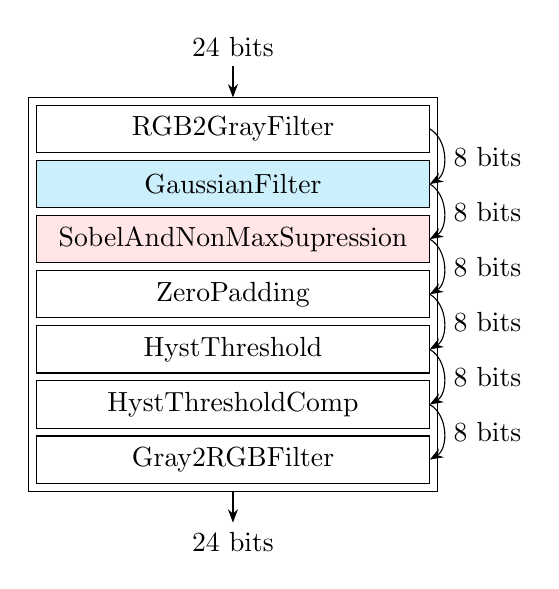
\begin{tikzpicture}
        \draw (-5.1,-2.5) rectangle (0.1,2.5);
        \fill[cyan!20] (-5,1.1) rectangle (0, 1.7);
        \fill[red!10] (-5,0.4) rectangle (0, 1.0);
        \foreach \x in {3,2,1,0,-1,-2,-3}
        {
            \draw (-5,{0.7*\x-0.3}) rectangle (0,{0.7*\x+0.3});
        }
        \node at (-2.5, 2.1) {RGB2GrayFilter};
        \node at (-2.5, 1.4) {GaussianFilter};
        \node at (-2.5, 0.7) {SobelAndNonMaxSupression};
        \node at (-2.5, 0) {ZeroPadding};
        \node at (-2.5, -0.7) {HystThreshold};
        \node at (-2.5, -1.4) {HystThresholdComp};
        \node at (-2.5, -2.1) {Gray2RGBFilter};
        \foreach \x in {2,1,0,-1,-2,-3}
        {
            \draw[-Stealth] (0, {0.7*\x+0.7}) to [bend left=60] node[right] {8 bits} (0, {0.7*\x});
        }
        
        \draw[-Stealth] (-2.5, 2.9) node[above] {24 bits} -- (-2.5, 2.5);
        \draw[-Stealth] (-2.5, -2.5) -- (-2.5, -2.9) node[below] {24 bits};
    \end{tikzpicture}
    \begin{itemize}
        \item \textcolor{cyan}{
             Gaussian Filter は8bitの5x5サイズの畳み込みで遅延。 }
        \item \textcolor{cyan}{
            3x3 サイズに落として計算。}
    \end{itemize}
\end{frame}



\begin{frame}{SobelAndNonMaxSupression の構成}
    \begin{columns}[t,onlytextwidth]
        \begin{column}{0.5\textwidth}
        SobelAndNonMaxSupression の構成
    \centering
    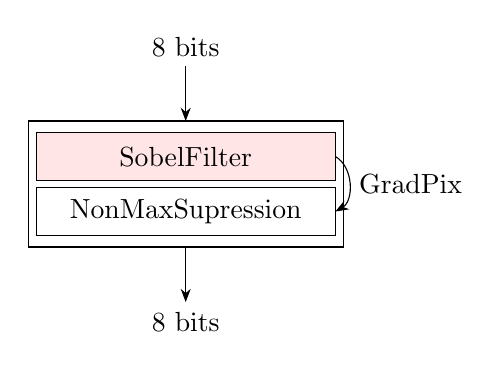
\begin{tikzpicture}
        \draw (-4.5,-0.8) rectangle (-0.5, 0.8);
        \fill[red!10] (-4.4, 0.05) rectangle (-0.6, 0.65);
        \foreach \x in {-1,1}
        {
            \draw (-4.4, {0.35*\x-0.3}) rectangle (-0.6, {0.35*\x+0.3});
        }
        \node at (-2.5, 0.35) {SobelFilter};
        \node at (-2.5, -0.35) {NonMaxSupression};
        \draw[-Stealth] (-0.6, 0.35) to [bend left=60] node[right] {GradPix} (-0.6,-0.35);  
        
        \draw[-Stealth] (-2.5, 1.5) node[above] {8 bits} -- (-2.5, 0.8);
        \draw[-Stealth] (-2.5, -0.8) -- (-2.5,-1.5) node[below] {8 bits};
   \end{tikzpicture} 
   \end{column}
   \begin{column}{0.5\textwidth}
        SobelFilterの構成
       \centering
       \begin{tikzpicture}
           \draw (-4.5, -1.1) rectangle (-0.5, 1.1);
           \only<1>{
                \fill[cyan!20] (-4.4, -0.3) rectangle (-0.6, 0.3);
           }
           \only<2>{
                \fill[olive!20] (-4.4, 0.4) rectangle (-0.6, 1.0);
           }
           \foreach \x in {-1,0,1}
           {
                \draw (-4.4, {0.7*\x-0.3}) rectangle (-0.6, {0.7*\x+0.3});
           }
           \node at (-2.5, 0.7) {SobelConvolution};
           \node at (-2.5, 0) {SqrtWrapper};
           \node at (-2.5, -0.7) {CalculateGradient};
           
           \draw[-Stealth] (-2.5, 1.9) node[above] {8bits} -- (-2.5, 1.1);
           \draw[-Stealth] (-2.5,-1.1) -- (-2.5, -1.9) node[below] {GradPix};
       \end{tikzpicture}
   \end{column}
   \end{columns}
   \only<1>{
        \textcolor{cyan}{
            32 bit の開平法は遅延するので、レジスタを導入。
        }
   }
   \only<2>{
        \textcolor{olive}{
            16 bit の3x3サイズの畳み込みが遅い可能性。
        }
   }
\end{frame}
\begin{frame}{Contents}
   \begin{itemize}
       \item[\textcolor{red}{$\checkmark$}] Chisel の導入
       \item[\textcolor{red}{$\checkmark$}] Pros. \& Cons.
       \item[\textcolor{red}{$\checkmark$}] ChiselImProc の説明
       \item[\textcolor{red}{$\rhd$}] Vivado HLS との比較
   \end{itemize} 
\end{frame}



\begin{frame}{Lenna の画像によるテストベンチ}
    \begin{columns}[t, onlytextwidth]
        \begin{column}{0.5\textwidth}
            Vivado HLS
            \begin{figure}
                \centering
                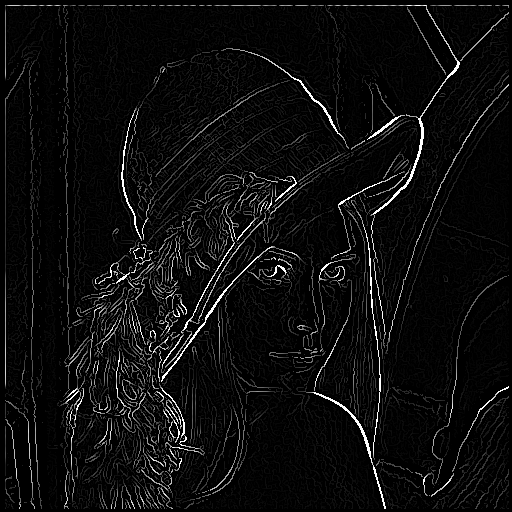
\includegraphics[width=0.9\textwidth]{./figures/out_hls.png}
            \end{figure}
        \end{column}
        \begin{column}{0.5\textwidth}
            Chisel
            \begin{figure}
                \centering
%                \begin{overpic}[grid,width=0.9\textwidth]{./figures/out_original.png}
%                \end{overpic}
                \only<1>{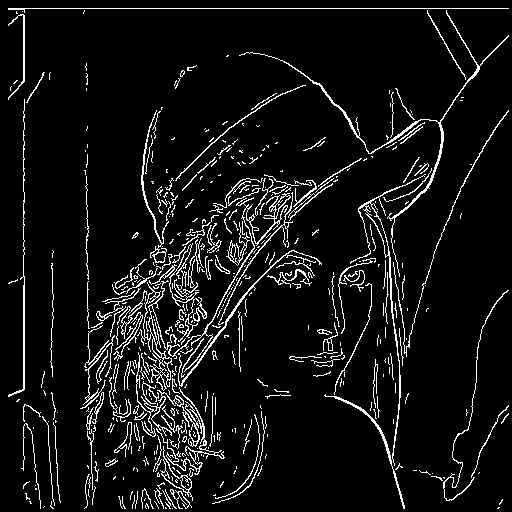
\includegraphics[width=0.9\textwidth]{./figures/out_original.png}}
                \only<2>{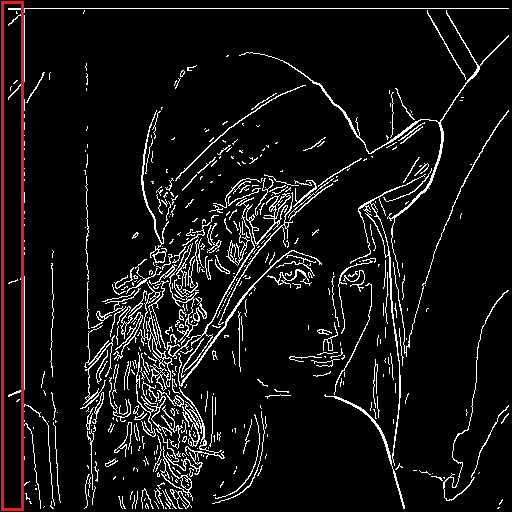
\includegraphics[width=0.9\textwidth]{./figures/out_original_edit.png}}
            \end{figure}
        \end{column}
    \end{columns}
    \begin{itemize}
        \item HLS のほうだとなぜか2値になっていない
        \item last信号の処理が甘いため20ピクセルほどずれる
    \end{itemize}
    
    
\end{frame}


\begin{frame}{Implementation後のUtilization}
\begin{columns}[t,onlytextwidth]
    \begin{column}{0.5\textwidth}
        Vivado HLS
        \begin{figure}
            \centering
            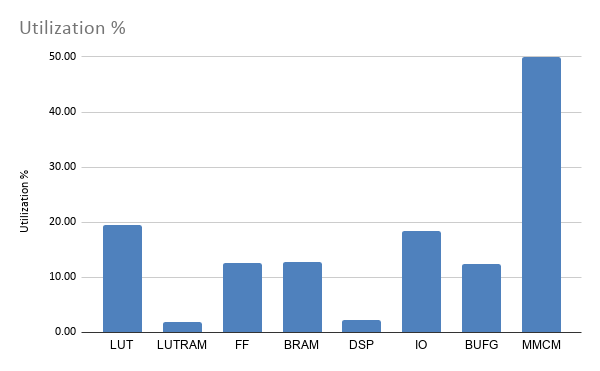
\includegraphics[width=\textwidth]{./figures/Utilization_hls.png}
        \end{figure}
    \end{column}
    \begin{column}{0.5\textwidth}
        Chisel
        \begin{figure}
            \centering
            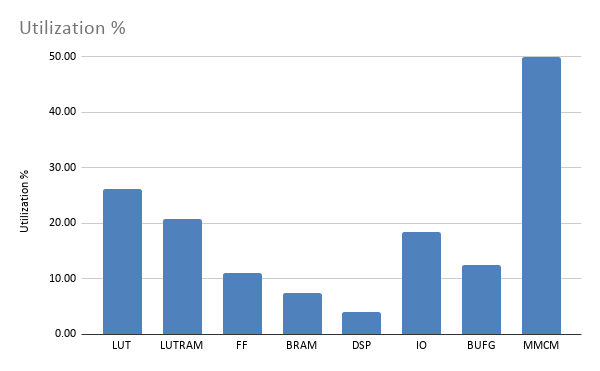
\includegraphics[width=\textwidth]{./figures/Utilization_chisel.png}
        \end{figure}
    \end{column}
\end{columns}

ChiselのBRAMはSystem ila ($+15 \sim 20$\%) が含まれる。
    
\end{frame}





\begin{frame}{参考文献}
    \begin{itemize}
        \item Digital Design with Chisel \\
            \scriptsize{
            \url{https://raw.githubusercontent.com/wiki/schoeberl/chisel-book/chisel-book.pdf}
            \url{https://github.com/schoeberl/chisel-book}
            }
            
        \item Chisel入門書「Digital Design with Chisel」1章の勉強記録 \\
            \scriptsize{
            \url{https://qiita.com/Kosuke_Matsui/items/80dde1219e3ce02c4b66}
            }
            
        \item Chisel 3 Wiki \\
            \scriptsize{
            \url{https://github.com/chipsalliance/chisel3/wiki}
            }
            
        \item Scala Doc \\
            \scriptsize{
            \url{https://www.chisel-lang.org/api/latest/chisel3/index.html}
            }
            
        \item Cheet Sheet \\
            \scriptsize{
            \url{https://github.com/freechipsproject/chisel-cheatsheet/releases/latest/download/chisel_cheatsheet.pdf}
            }
    \end{itemize}
\end{frame}

\end{document}
